\chapter{Background \& Theory} \label{chap:2}
 
In modern \gls{DoD} air combat operations, collateral damage and aircraft survivability estimates significantly influence the tactics and procedures utilized during any given attack mission. Consequently, military commanders and weaponeering experts must prepare armament packages which present the smallest amount of risk to civilian populations and structures, while exposing the least amount of military personnel and assets to hostile environments. Currently, the \gls{DoD} and \gls{USAF} are unable to custom build weapons for specific targets in a timely and efficient manner, meaning most missions rely on ready-made munitions not designed for unique circumstances. 

Modern military aircraft armament is produced using traditional metal processing methods, such as forging or casting. These techniques feature pre-determined molds or shaping instructions which require machine and assembly downtime to modify, making them unsuited for frequently changing requirements. By contrast, \gls{AM} enables manufacturers to customize and adjust part dimensions and features to customer requirements. Applying this to military weaponeering, \gls{AM} provides a potential solution to materializing a customized bomb-building capability. Since \gls{AM} and warhead design are largely studied independent of one another, there is little documentation on how \gls{AM}-printed metals respond to explosive detonations. This research seeks to investigate the performance of additively manufactured metal casings undergoing explosive loading. Classic fragmentation theories developed by R.W. Gurney and N.F. Mott provide a foundation to characterize experimental results and compare additively manufactured casing performance with traditional metal production methods. High speed photography and subsequent \gls{DIC} analysis visually capture and quantify the metal's mechanical properties, bringing awareness to \gls{AM}'s suitability in weaponeering applications.



%-----------------------------------------------------------------------
\section{Additive Manufacturing} \label{sec:2_AdditiveManufacturing}
%-----------------------------------------------------------------------

\gls{AM} is an umbrella term used to describe fabrication techniques which produce components through a progressive layering process. Colloquially referred to as ``3D printing," \gls{AM} is becoming increasingly common in a wide array of industries as it becomes a more economical and reliable production method. Although there are several different types of \gls{AM} processes, each having its own construction method and resulting material characteristics, \gls{PBF} was selected for this research.

% Although there are several different types of \gls{AM} processes, each having its own construction method and resulting material characteristics, \gls{SLM} was selected for this research.

%%%%%%%%%%%%%%%%%%%%%%%%%%%%%%%%%%%%
\subsection{\glsentryfull{PBF}} \label{sec:2_PBF}
%%%%%%%%%%%%%%%%%%%%%%%%%%%%%%%%%%%%

% %%%%%%%%%%%%%%%%%%%%%%%%%%%%%%%%%%%%
% \subsection{Selective Laser Melting} \label{sec:2_SLM}
% %%%%%%%%%%%%%%%%%%%%%%%%%%%%%%%%%%%%

\gls{PBF} machines, illustrated in \Cref{fig:2_PBF_Setup}, fabricate parts in a successive layering system using deposited powder and a directional laser heat source. First, a desired part's \gls{CAD} model is uploaded into the \gls{PBF} machine, which divides the model into cross-sectional layers, converting it into a series of individual layer blueprints. For each layer, the machine then maps the optimal laser path needed to achieve a desired level of quality, creating the overall scan strategy.

% \gls{SLM} machines, illustrated in \Cref{fig:2_SLM_Setup}, fabricate parts in a successive layering system using deposited powder and a directional laser heat source. First, a desired part's \gls{CAD} model is uploaded into the \gls{SLM} machine, which divides the model into cross-sectional layers, converting it into a series of individual layer blueprints. For each layer, the machine then maps the optimal laser path needed to achieve a desired level of quality, creating the overall scan strategy.

% PBF Machine Illustration
\begin{figure}[H]
	\centering
 \fbox{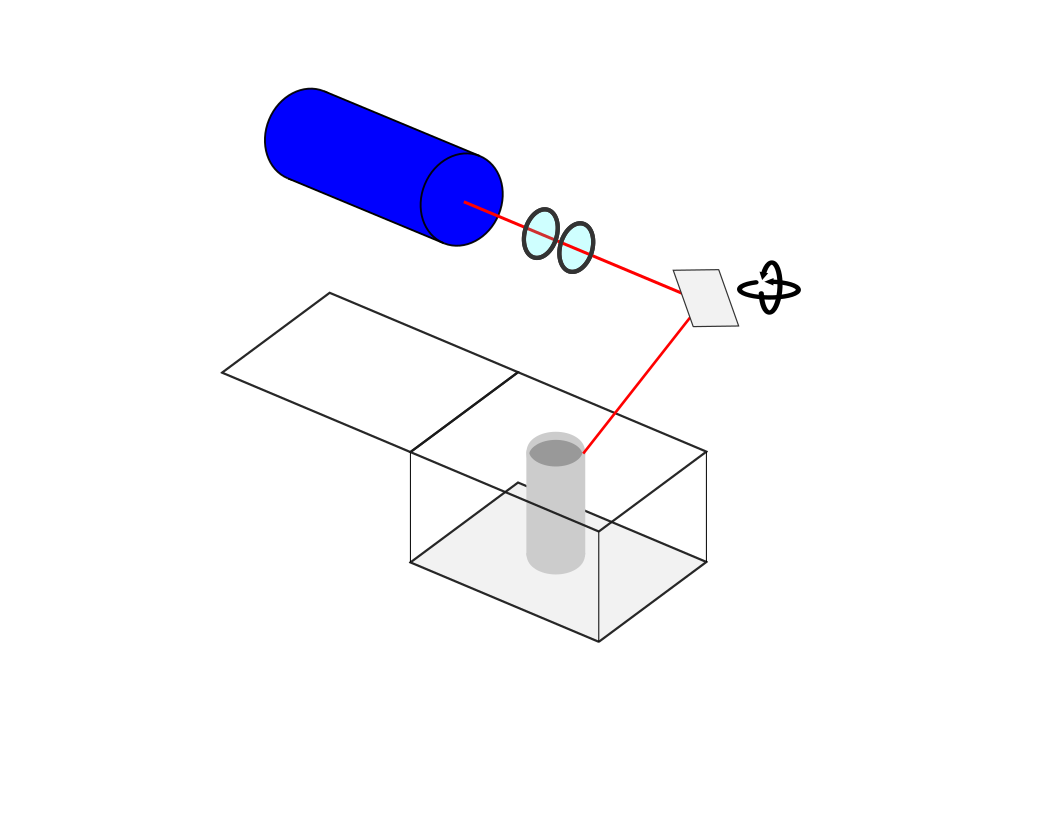
\includegraphics[width=0.7\linewidth]{Ch2/Figures/PBF_Setup.png}}
    \caption{Illustration of an \gls{PBF} machine, based on an illustration presented in \textit{The metallurgy and processing science of metal additive manufacturing} \cite{OverviewofAM_OHara} 
    \textbf{rough draft note: I am still working on drawing this, so it is incomplete}}
	\label{fig:2_PBF_Setup}
\end{figure}
%

Once the \gls{PBF} machine generates a manufacturing solution, an emitted laser is guided along the build path using a lens configuration and scanning mirror. The laser's energy rapidly heats and melts the deposited powder, which forms a solid layer upon cooling. After the laser completes the layer's build path, the powder platform is raised while the build platforms lowers by the length of one layer thickness. Next, the recoater blade spreads a layer of powder metal across the build platform, depositing new material on top of the previously scanned layer. The laser then maneuvers along the ensuing layer's build path, and the process is repeated until the entire part is constructed \cite{OverviewofAM_OHara}.

One of the most common \gls{PBF} techniques is \gls{DMLS}, a laser-based \gls{AM} method attributed to metal \gls{PBF} systems built by the German company EOS GmbH. Although they are named after the sintering process (fusing materials at temperatures slightly below their melting temperature) originally used by first generation printers in the mid-1990's, modern \gls{DMLS} manufacturing completely melts the deposited powder (EOS, private communication), making it equivalent to \gls{SLM} \cite{EOS_DMLS_History}.  

The primary advantage of \gls{DMLS} over sintering-based \gls{PBF} techniques, such as \gls{SLS}, is its ability to achieve relative densities of approximately 100 \% \cite{EOS_StainlessSteel_M290}. Compared to \gls{DMLS}, \gls{SLS} uses lower powered lasers which do not fully melt the build material, resulting in lower density components with inferior strength properties \cite{SLS_not_fully_dense}. Since \gls{DMLS} is a metal-based \gls{AM} technique, commonly used powders include aluminum, nickel, stainless steel, and titanium-based alloys. ...For high temperature and stress applications, 15-5 \gls{PH} stainless steel...

%Paragraph on 15-5 powder
15-5 \gls{PH} stainless steel is a martensitic steel alloy originally designed by Aramco (now AK Steel) as an improved variation of 17-4 \gls{PH} stainless steel. Since it lacks the weaker ferrite crystal structure found in 17-4 \gls{PH} stainless steel, 15-5 \gls{PH} stainless steel exhibits favorable strength properties  \cite{AKSteel_Conventional_SS,Ferrite_weaker}.
Following construction completion, 15-5 \gls{PH} stainless steel components are typically heat treated at a temperature between 900 and 1150 \degree F, significantly strengthening the components at a slight expense to material ductility \cite{AKSteel_Conventional_SS,EOS_StainlessSteel_M290}.  

%Unlike  sintered , \gls{DMLS} parts feature near full density

%%%%%%%%%%%%%%%%%%%%%%%%%%%%%%%%%%%%
\subsection{Powder Bed Fusion Drawbacks} \label{sec:2_PBF_drawbacks}
%%%%%%%%%%%%%%%%%%%%%%%%%%%%%%%%%%%%
While \gls{PBF} gives the manufacturer significant control over design parameters, the presence of a continuously-moving heat source (laser) introduces several sources of variability not found in conventional machining methods. For instance, prior research has shown variations in laser scan speed alone can have profound effects on the final part's porosity levels \cite{ChoiSLMDensity}. Additionally, entrapped gases, as well as size and shape variations in the powder feedstock further promote micropore formation \cite{Aboulkhair2014_microscopic_pores}. Other possible issues in \gls{PBF} include delamination (layer separation), cracking, and residual stress buildup. The presence and frequency of effects is controlled by laser power, powder feedstock quality, scan strategy, and various \gls{PBF} machine parameters \cite{OverviewofAM_OHara}. Together, these imperfections weaken the printed component's overall strength, which translates to impacting the casing's ability to withstand explosive loadings in this research.

Roberts et al. tensile tested \gls{DMLS} and wrought 15-5 \gls{PH} stainless steel cylindrical rods at elevated temperatures (593 \degree C) and noted while \gls{DMLS}-printed samples exhibited superior yield strength (...MPa vs ...Mpa) and ultimate tensile strength (...MPa vs ...Mpa) values, wrought samples displayed greater elongation percentages at fracture (..\% vs ..\%), suggesting \gls{DMLS} processing reduces material ductility \cite{Roberts_Traditional_AM_15_5_testing}. 

% PBF Machine Illustration
\begin{figure}[H]
	\centering
 \fbox{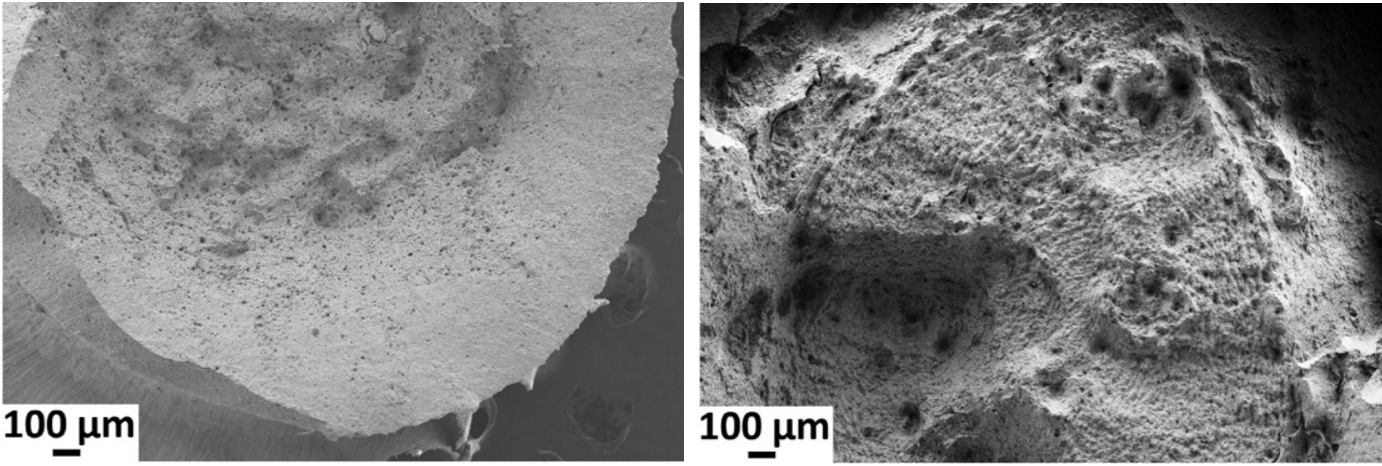
\includegraphics[width=0.7\linewidth]{Ch2/Figures/Wrought_vs_DMLS.PNG}}
    \caption{Comparison of wrought (left) and DMLS (right) test...Image adapted from \textit{A comparative study of microstructure and high-temperature mechanical properties of 15-5 PH stainless steel processed via additive manufacturing and traditional manufacturing}\cite{Roberts_Traditional_AM_15_5_testing}.} 
    \label{fig:2_Wrought_vs_DMLS_fracture surface}
\end{figure}
%


%Carlton et al. discovered SLM-printed stainless steel specimens with high porosity concentrations (> 2%) undergoing tensile testing fail in...under tension, while low porosity samples (< 1%) samples exhibit...failure (\ ....additionally, porosity increases.... [damage evolution and failure mechanisms...] as 

%-----------------------------------------------------------------------
\section{Warhead Performance \& Fragmentation Theories} \label{sec:2_Warhead_Fragmentation_Theories}
%-----------------------------------------------------------------------

A fragmenting warhead's effectiveness and lethality are primarily determined by the casing's material performance under the explosive loading. For instance, when a warhead detonates, the generated shock wave travels outward into the casing until reaching the casing's free surface with the atmosphere. At this point, a rarefaction (relief) wave reflects back into the casing until it reaches the inner wall surface, reflecting a shock wave back towards the outer surface. This wave reflection process continues to repeat, accelerating the casing outward, until the casing fractures \cite{Blast_injury_science_shockwave}. Since this creates an extremely fast and complex explosive event, experts continually try to simplify underlying physics using analytical expressions and models. One of the most widely used formulas for predicting a warhead's fragmentation velocity is the Gurney equation.  

%AM defects could impede the shockwave's transmission through the casing, decreasing it's overall contribution to material deformation.

%Voids may serve as local free surfaces, creating additional reflected waves within the casing itself.
%.....shockwaves accelerate

%Additive Manufacturing ductility comparison...fragment's accelerated 
%%%%%%%%%%%%%%%%%%%%%%%%%%%%%%%%%%%%
\subsection{Gurney Equation} \label{sec:2_Gurney}
%%%%%%%%%%%%%%%%%%%%%%%%%%%%%%%%%%%%
In the 1940s, R. W. Gurney researched fragmentation velocity of various military munitions at Ballistics Research Laboratories, located at Aberdeen Proving Grounds, MD.
Using a velocity camera positioned approximately 9 feet from the target, Gurney measured the initial fragment velocity of various types of explosive weapons. Gurney also employed a conservation of energy approach to mathematically characterize these detonations, concentrating on chemical-to-kinetic energy conversion to determine velocity of resulting fragments.

%Assumptions 
The kinetic energy $K$ of object $i$ is a function of its mass $m$ and velocity $V$, as shown in the fundamental equation below:
%Eq: Fundamental KE equation
\begin{equation}
K_{i} = \frac{1}{2}m_{i}{V_{i}}^2
\label{eq:2_KE}
\nomenclature{K}{Kinetic Energy}
\nomenclature{V}{Velocity}
\nomenclature{m}{Mass}
\end{equation}
%
Gurney hypothesized the amount of kinetic energy generated by detonating a unit mass of explosive is independent of projectile size; therefore, initial fragmentation velocity $V_0$ is not a function of the warhead's dimensions. Since detonations are dynamic events featuring multiple energy conversion stages over a short timespan, Gurney made several key assumptions to simplify the warhead detonation's underlying physics.

First, Gurney refined the conservation of energy principle and assumed all chemical energy provided by the explosive mass instantly converts to kinetic energy upon detonation, neglecting the work required to rupture the casing and all other energy conversion events occurring during the explosion. Therefore, the total amount of the energy per unit length of explosive is equal to the product of the explosive's specific energy $E$ and mass per unit length $C$. Since the casing and explosive masses both have kinetic energy after detonation, Gurney set the summation of these values equal to $EC$, as shown below: 
%Eq - Total KE in System 
\begin{equation}
EC = K_{Explosive} + K_{Casing}
\nomenclature{$E$}{Explosive Specific Energy}
\nomenclature{$C$}{Explosives Mass}
\label{eq:2_Overall_EC}
\end{equation}
%
where $K_{Explosive}$ and $K_{Casing}$ are the amounts of kinetic energy per unit length for the explosive and casing products, respectively. 

For the expanding detonation gases, Gurney assumed a uniform velocity distribution along the cylinder's entire length. This assumption is not valid in reality due to end effects, which are covered in further detail later in this section \cite{GurneyOriginal}. Additionally, Gurney assumed a linear velocity gradient in the radial direction, from the cylinder's centerline ($V_{r=0} = 0$) to its inner wall ($V_{r=a} = V_0$), as depicted in \cref{fig:2_Cylinder_V_r} below: 
%Fig - Velocity Gradient
\begin{figure}[H]
	\centering
 \fbox{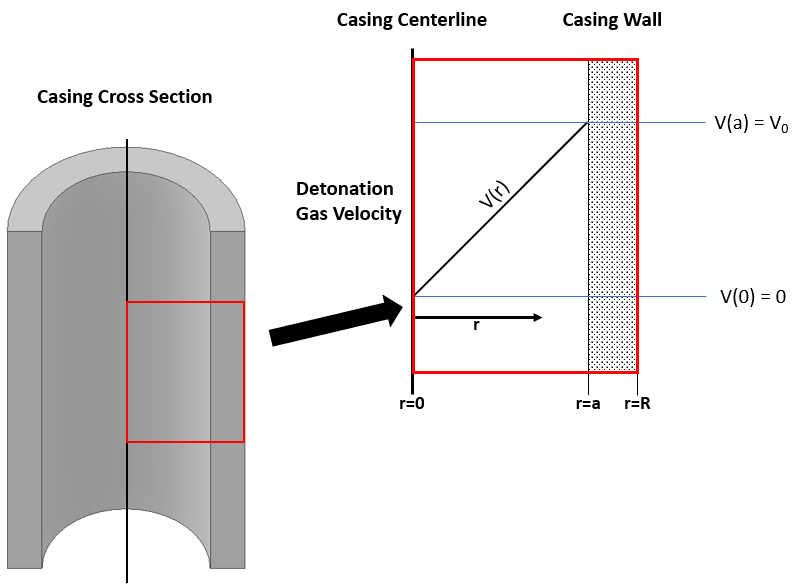
\includegraphics[width=0.7\linewidth]{Ch2/Figures/Cylinder_V_r.PNG}}
    \caption{Visual depiction of linear velocity gradient assumed by Gurney, 	based on an illustration from \textit{Gurney Energy of Explosives: Estimation of the Velocity and Impulse Imparted to Driven Metal} \cite{GurneyKennedy1970}}
	\label{fig:2_Cylinder_V_r}
\end{figure}
%
Consequently, the detonation velocity at any position within the casing is a function of distance from the cylinder's longitudinal axis, $r$,
%
\begin{equation}
V(r) = \frac{r}{a}V_0
\label{eq:2_linearvelocity}
\end{equation}
%

Another key assumption Gurney made was a constant density $\rho$ in the detonation product gases \cite{GurneyOriginal}. When the explosive is treated as a unit length cylinder with outer radius $a$ (casing inner radius), its density is then:
%Eq - Explosives density
\begin{equation}
\rho = \frac{C}{\pi{a^2}}
\label{eq:2_explosive_density}
\end{equation}
%
Furthermore, the volume $\volume$ for any portion of the unit length cylinder between $r$ and $r+dr$ (depicted in \Cref{fig:2_Cylinder_dr_calculation}) is: 
%Eq - Vol of cylinder portion
\begin{equation}
\volume = 2\pi{r}dr
\label{eq:2_unitcylindervolume}
\end{equation}
%
%Fig - Picture showing dr portion of explosive
\begin{figure}[H]
	\centering
 \fbox{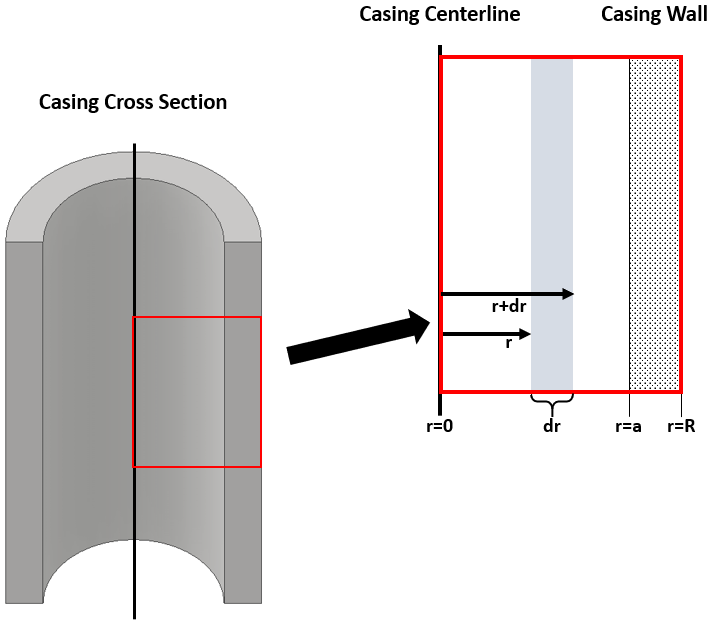
\includegraphics[width=.6\linewidth]{Ch2/Figures/Cylinder_dr_calculation.PNG}}
    \caption{Illustration portraying volume $\volume$ calculation in \Cref{eq:2_unitcylindervolume}, based on a drawing from \textit{ESTIMATION OF VELOCITY DISTRIBUTION OF FRAGMENTING WARHEADS USING A MODIFIED GURNEY METHOD} \cite{AFIT_Yves}}
\label{fig:2_Cylinder_dr_calculation}
\end{figure}
%
The explosive mass per unit length $C$ is determined by integrating \Cref{eq:2_unitcylindervolume} from the unit cylinder's center ($r = 0$), to its inner wall ($r = a$), and multiplying by $\rho$:
%
\begin{align}
C &= \rho\int_{0}^{a}\volume \nonumber \\
C &= \rho\int_{0}^{a}2\pi{r}dr
 \label{eq:2_Casingmassintegral}
\end{align}
%Eq -  KE Explosive Mass
Inserting \Cref{eq:2_linearvelocity,eq:2_Casingmassintegral} into  \Cref{eq:2_KE}, $K_{Explosive}$ becomes
\begin{align}
K_{Explosive} &= \frac{1}{2}CV(r)^2 \nonumber \\
&= \frac{1}{2} {\underbrace{\rho\int_{0}^{a}2\pi{r}dr}_\textrm{Mass term}}
{\underbrace{\vphantom{\int_{0}^{a}}\Big(\frac{r}{a}V_0\Big)^2}_\textrm{Velocity term}} \nonumber \\
 &= \rho\pi{V_0}^2\int_{0}^{a}\frac{r^3}{a^2}dr \nonumber \\
K_{Explosive} &= \frac{\rho\pi{V_0}^2{a^2}}{4}
\label{eq:2_K_explosive_density}
\end{align}
Using \Cref{eq:2_explosive_density}, \Cref{eq:2_K_explosive_density} is rewritten in terms of $C$:
%
\begin{align}
K_{explosive} &= \frac{C}{\pi{a}^2} \frac{\pi{V_0}^2{a^2}}{4} \nonumber \\
K_{explosive} &= \frac{C{V_0}^2}{4}\label{eq:2_K_explosive_mass} 
\end{align}
%
%Eq -  KE of Casing
Since Gurney assumed a constant fragmentation velocity $V_0$ in the metal cylinder, $K_{casing}$ is obtained using \Cref{eq:2_KE}  
\begin{equation}
K_{casing} = \frac{1}{2}M{V_0}^2
\label{eq:2_KE_casing}
\end{equation}
%
\Cref{eq:2_K_explosive_mass,eq:2_KE_casing} are inserted into \Cref{eq:2_Overall_EC}, relating the kinetic energy terms to the explosive's stored chemical energy. Rearranging variables results in \Cref{eq:2_finalGurney}, also known as the Gurney equation for cylindrical casings, 
%
\begin{align}
EC &= \underbrace{\frac{C{V_0}^2}{4}}_\textrm{$K_{Explosive}$}  + \underbrace{\frac{1}{2}M{V_0}^2}_\textrm{$K_{Casing}$} \nonumber \\
EC &= {V_{0}}^2\Big(\frac{C}{4} +\frac{M}{2} \Big) \nonumber \\
\frac{1}{V_{0}^2} &= \frac{1}{EC}  \Big(\frac{C+2M}{4} \Big) \nonumber \\
\frac{1}{V_{0}^2} &= \frac{1}{2E}  \Big(\frac{1}{2} + \frac{M}{C} \Big) \nonumber \\
{V_{0}^2} &= \frac{2E}{  \Big(\frac{1}{2} + \frac{M}{C} \Big)} \nonumber \\
{V_{0}^2} &= 2E\frac{\frac{C}{M}}{  \Big(1 + \frac{1}{2}\frac{C}{M} \Big)} \nonumber \\
{V_{0}} &= \sqrt{2E} \sqrt{\frac{\frac{C}{M}}{1 + \frac{1}{2}\frac{C}{M}}} 
\label{eq:2_finalGurney}
\nomenclature{$M$}{Casing Mass}
\nomenclature{$a$}{Cylinder Inner Radius}
\nomenclature{$R$}{Cylinder Outer Radius}
\nomenclature{$V_{0}$}{Initial Fragment Velocity}
\end{align}
%
where the Gurney Velocity Coefficient $\sqrt{2E}$ (or Gurney Constant) is calculated using the explosive's specific energy $E$, and has units of velocity. Additionally, \Cref{eq:2_finalGurney} features the explosive charge to metal mass ratio $C/M$, which is determined by casing dimensions and explosive density. Therefore, all variables in the Gurney equation are controlled by the experimental design, making it an effective comparison method for analyzing test results.  

Although the Gurney equation provides an uncomplicated method for calculating fragmentation velocity, it utilizes several assumptions which are not always practical in real world applications. For instance, since Gurney derived \Cref{eq:2_finalGurney} from a unit length cylinder, there is no way to incorporate the casing's length to diameter ratio $L/D$. Since Gurney's report was published, subsequent research revealed fragments formed around the ends of detonating cylindrical warheads with $L/D$ ratios $\leq$ 2 exhibited fragmentation velocities much lower than predicted by the Gurney equation \cite{AFIT_Yves}. This phenomenon is now referred to as ``end effects."
\nomenclature{L/D}{length to diameter ratio}

End effects occur due to interactions between shock waves and rarefaction (relief) waves. Warheads are commonly designed with a single detonator located at one end of the cylinder. When the cylinder is detonated, shock waves develop and propagate away from the detonator location. Upon reaching the free surface between the casing and surrounding environment (air), rarefaction (relief) waves form, reflecting back into the casing and detonating explosive. Since a rarefaction wave lowers the pressure of the substance it travels through, it decreases the amount of loading available to expand the casing outward, inevitability lowering the fragmentation velocity.

Since the detonation is not instantaneous, it takes a finite amount of time for the chemical reaction process to travel down the entire length of the explosive filling. As a result, fragments located near the detonation end of the cylinder form rarefaction (relief) waves as the explosive is detonating, resulting in lower local fragment velocities. Analytical modeling of exploding TNT-filled cylinders in \textit{A Parametric Investigation and Optimization of a Cylindrical Explosive Charge}, illustrated in \cref{fig:2_Sawtooth_waves}: 
%Figure showing detonation/rarefaction wave interaction
\begin{figure}[H]
	\centering
 \fbox{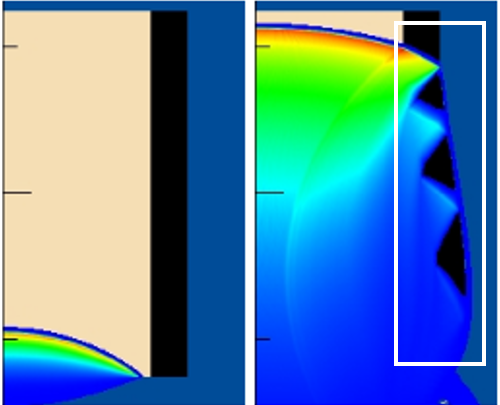
\includegraphics[width=0.6\linewidth]{Ch2/Figures/Beaver_End_Effects.PNG}}
    \caption{Two images depicting the evolution of a detonation wave in TNT (tan region), where the white box indicates the rarefaction/detonation wave interaction region .Image adapted from \textit{A Parametric Investigation and Optimization of a Cylindrical Explosive Charge} \cite{MarquetteEndEffects}.}
	\label{fig:2_Sawtooth_waves}
\end{figure}
%
Additionally, the shock wave generated by the detonator travels through the explosive filling and reaches the opposite end of the cylinder before the chemical reaction process is complete, creating more rarefaction waves at the far end's free surface. Consequently, in cylindrical warheads with low $L/D$ values, reduced fragmentation velocities also occur at the opposite end of the detonator \cite{AFIT_Yves,MarquetteEndEffects}. This phenomenon manifested in experiments conducted by Huang and Feng, where a cylinder with $L/D$ = 1.3 was detonated, producing the fragmentation velocity profile shown in \Cref{fig:2_end_effects} below \cite{HuangEndEffects}:    
%Figure showing impact of end effects on fragmentation velocity
\begin{figure}[H]
	\centering
 \fbox{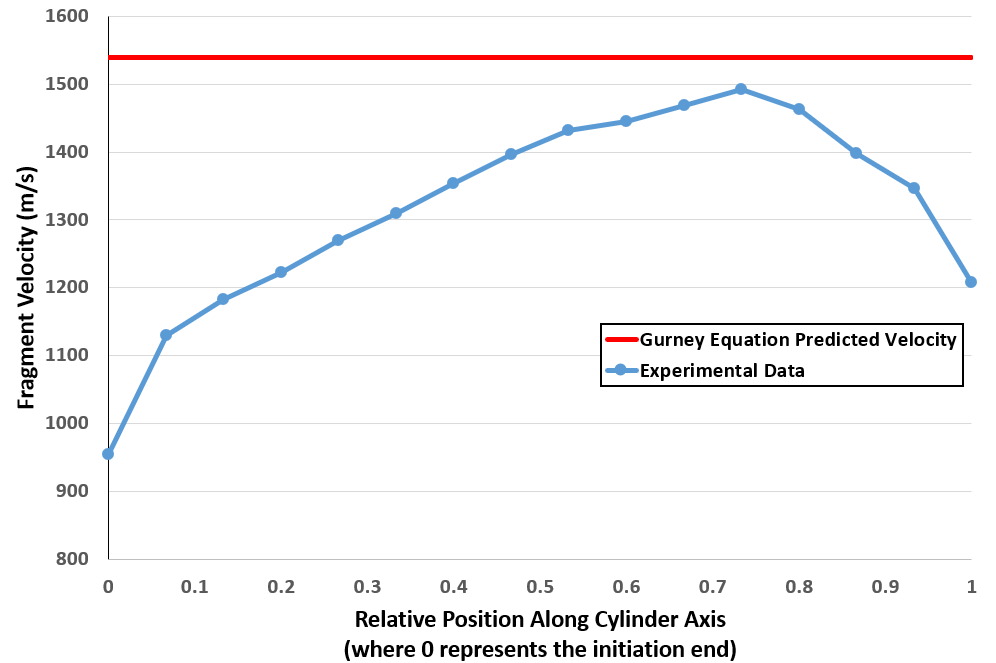
\includegraphics[width=0.7\linewidth]{Ch2/Figures/End_Effects.PNG}}
    \caption{Experimental data from \textit{Axial distribution of Fragment Velocities from cylindrical casing under explosive loading} showing the influence of end effects during fragmentation events \cite{HuangEndEffects}.}
	\label{fig:2_end_effects}
\end{figure}
%
\cref{fig:2_end_effects} compares Huang and Feng's measured data with the corresponding Gurney equation prediction. Near the initiation end (0 on the horizontal axis), shock and relief wave interactions (as shown in \cref{fig:2_Sawtooth_waves}) result in fragmentation velocities significantly lower than predicted by the Gurney equation. Similarly, the rarefaction waves formed after the initial detonation wave reaches the cylinder's far end (1 on the horizontal axis) weaken the local pressure loadings generated by the ongoing explosive filling detonation, reducing far end casing expansion rates and the resulting fragmentation velocities.

%Gurney equation doesn't account for material properties
Another Gurney equation limitation is its inability to account for casing material properties. 
%%%% Include copper steel graph

%and concluded the initial detonation wave notably contributes to casing acceleration. 
\cite{WangDuctilityExpansion}


In addition to fragmentation velocity, weapons developers also use fragment mass distribution to characterize the potential damage caused by exploding warheads. Some weapons even feature ``pre-fragmented" designs, controlling the resulting fragments' size and shape \cite{DrielsWeaponeering}. While many fragmentation studies have transitioned to computer-based modeling to exploit high performance computer capabilities \cite{GrisaroFragmentVelocityDistribution,MarquetteEndEffects,MoxnesRingFragmentationSimulation}, most researched is derived from N.F. Mott's fragmentation theory. 
%%%%%%%%%%%%%%%%%%%%%%%%%%%%%%%%%%%%
\subsection{Mott Fragmentation Model}
%%%%%%%%%%%%%%%%%%%%%%%%%%%%%%%%%%%%

%Due to the layering scheme present in AM,....Mott fragmentation distribution cannot be applied from a length perspective


In early 1940s England, N.F. Mott began studying warhead fragmentation to support the ongoing World War II effort. Through a series of reports, Mott attempted to model the weight distribution of fragments created by exploding bombs and shells. In 1943, he developed two scaling relations for fragmenting cylindrical shells, giving weapons developers the ability to study the effects of modifying warhead dimensions without conducting experimental tests \cite{GradyMottLegacy}.     
The following distribution predicts the number of fragments $n(m)$ with weights between $m$ and $m + dm$: 
%
\begin{equation} %page 141,228 - Grady ; Fragmentation of HE Shells
	dN = B\exp\bigg({-\frac{\sqrt{m}}{M_{A}}}\bigg)d\sqrt{m}
    \label{eq:2_Mott1943_dN}
\end{equation}
%
where $M_{A}$ is defined as
%
\begin{equation} 
	M_{A} = {\Gamma}t^{\nicefrac{5}{6}}d_{in}^{\nicefrac{1}{3}}\Big(1+\frac{t}{d_{in}}\Big) 
    \label{eq:2_Mott1943Ma}
\end{equation}
%
In \Cref{eq:2_Mott1943_dN,eq:2_Mott1943Ma}, $m$ is the fragment mass, $B$ is a distribution factor, and $\Gamma$ is an empirical constant based on explosive properties, and $d_{in}$ and $t$ are the casing's inner diameter and thickness, respectively. Next, fragment mass distribution $dM$ is obtained by multiplying \Cref{eq:2_Mott1943_dN} by $m$:
%Eq:dM - ma
\begin{align}
dM &= mdN \nonumber \\
dM &= mB\exp\bigg({-\frac{\sqrt{m}}{M_{A}}}\bigg)d\sqrt{m}
 \label{eq:2_Mott1934_dM}
\end{align}
%
Since the sum of the fragment masses is equal to the casing mass $M$, $B$ is calculated using integration by parts $\int{udv} = uv - \int{vdu}$: 
%Eq - B Derivation
\begin{align}
M &= \int_{0}^{\infty}dM \nonumber \\
 &= B\int_{0}^{\infty}m\exp\bigg({-\frac{\sqrt{m}}{M_{A}}}\bigg)d\sqrt{m}
\nonumber \\
 &= B\int_{0}^{\infty}x^{2}e^{-\tfrac{x}{y}}dx \text{\phantom{..............} where $x = \sqrt{m}$ and $y = M_{A}$} 
\nonumber \\ 
 &= B\bigg[-ye^{-\tfrac{x}{y}}x^2+\int{2y}e^{-\tfrac{x}{y}}xdx\Bigg]_{0}^\infty \nonumber \\
 &= B\bigg[-ye^{-\tfrac{x}{y}}x^2+{2y}\Big(-ye^{-\tfrac{x}{y}}x+\int{ye^{-\tfrac{x}{y}}}dx\Big)\Bigg]_{0}^\infty \nonumber \\
 &= B\bigg[-ye^{-\tfrac{x}{y}}x^2+{2y}\Big(-ye^{-\tfrac{x}{y}}x-{y^2e^{-\tfrac{x}{y}}}\Big)\Bigg]_{0}^\infty \nonumber \\
 &= B(0-(-2y^3)) \nonumber \\
M &= 2B{M_{A}}^3 \nonumber \\
B &= \frac{M_0}{2{M_{A}}^3}
\label{eq:2_Mott1934_B}  
\end{align}
%
Mott's cumulative fragment distribution is obtained by integrating \Cref{eq:2_Mott1943_dN} and substituting in \Cref{eq:2_Mott1934_B} to incorporate material properties:
%Eq - Cumulative Fragment Distribution
\begin{align}
N(m) &= \int_{m}^{\infty}dN \nonumber \\
 &= B\int_{m}^{\infty}\exp\bigg({-\frac{\sqrt{m}}{M_{A}}}\bigg)d\sqrt{m} \nonumber \\
&= \frac{M_0}{2{M_{A}}^3}\int_{m}^{\infty}\exp\bigg(-{\frac{\sqrt{m}}{M_{A}}}\bigg)d\sqrt{m}
\nonumber \\
&= \frac{M_0}{2{M_{A}}^3}\bigg[-M_{A}\exp\bigg(-\frac{\sqrt{m}}{M_{A}}\bigg) \bigg]_{m}^\infty  \nonumber \\
&= \frac{M_0}{2{M_{A}}^3}\bigg(0 - \bigg(-M_{A}\exp\bigg(-\frac{\sqrt{m}}{M_{A}}\bigg)\bigg) \bigg)  \nonumber \\
N(m) &= \frac{M_0}{2{M_{A}}^2}\exp\bigg(-\frac{\sqrt{m}}{M_{A}}\bigg)
\label{eq:2_Mott1934_Cumulative_frag}  
\end{align}
%
where $N(m)$ is the number of resulting fragments with a mass greater than $m$.

In \textit{Fragmentation of shell cases}, Mott noted exploding forged steel shells typically fracture in segments running parallel to the casing's longitudinal axis, forming large, thin fragments \cite{Mott1947}. This is likely due to the largely homogeneous composition found in conventionally produced metals, meaning the casing does not have any substantial weak points prone to early failure. By contrast, the additively manufactured metals featured in this research have inherent flaws by nature of the manufacturing process (as covered in \Cref{sec:2_SLM_drawbacks}). The use of a layering construction process and localized heat source in \gls{DMLS} creates a non-uniform distribution of internal features (micropores, melt pool boundaries, etc.) along the part's build direction. As shock waves and detonation product gases exert loadings on these weakened imperfections, they may prematurely fracture, causing the cylinder casing to fail.

Similar to the Gurney equation, the Mott fragmentation model also lacks a variable to readily account for the casing's material properties. 
 In Mott's original work, the munitions' mild steel casings properties were incorporated into empirically derived $\Gamma$ values \cite{Mott_Fragmentation_DOE}. While this was largely sufficient for predicting fragmentation characteristics of weapons used during the 1940s, there is no empirical solution for the wide array of materials featured in modern weapons.
 Although the fragmentation theories presented in \Cref{sec:2_Warhead_Fragmentation_Theories} are extremely useful analytical tools, experimental testing is still an essential element of weapons design. Unfortunately, explosives testing features extremely fast detonation rates are not observable to the naked eye and common optical equipment. Therefore, to maximize data collected during testing, specialized diagnostic methods are used to witness the entire process.   

%-----------------------------------------------------------------------
\section{Diagnostic Techniques} \label{sec:2_Diagnostic_Techniques}
%-----------------------------------------------------------------------


%%%%%%%%%%%%%%%%%%%%%%%%%%%%%%%%%%%%
\subsection{High Speed Photography} \label{sec:2_Diagnostic_Photography}
%%%%%%%%%%%%%%%%%%%%%%%%%%%%%%%%%%%%

Since explosions involve extremely fast chemical reaction rates (typical detonation velocities in air are 5-10 km/s) \cite{Cooper1996}, cylinder casing fractures occurs within tens of microseconds of detonation \cite{ExpandingFractureBehavior1045Cylinder}.
%, if visual investigations are desired.
%Historical high speed photography relied on…
%Modern high speed cameras store….directly on, enabling frame rates of X million \gls{fps}
Fortunately, modern high speed cameras store….directly on, enabling frame rates on the order of millions of \gls{fps}. Unlike other high speed recording techniques, such as \gls{DPV} and Flash Radiograph, which involve complex, specialized support equipment, high speed cameras only require a calibrated lighting source and computer interface for camera synchronization.   
%. While these methods can achieve...(very accurate results?), they are typically limited to analyzing...(one surface?) and require specialized test equipment. For instance, 

%%%%%%%%%%%%%%%%%%%%%%%%%%%%%%%%%%%%
\subsection{\glsentryfull{DIC}} \label{sec:2_Diagnostic_DIC}
%%%%%%%%%%%%%%%%%%%%%%%%%%%%%%%%%%%%
\gls{DIC} is a non-contact optical tracking method used to capture the deformation and displacement of materials in motion. This is accomplished by comparing the movement of small pixel groups ``subsets" over a series of images. Since the software's accuracy is determined by its ability to identify and trace pixel movements, both the test specimen and its surrounding environment must be specially prepared for optimal data collection conditions. This is typically done by coating a portion of the test specimen with a speckle pattern for the \gls{DIC} software to identify and track.

Over the past 20 to 25 years, \gls{DIC} has emerged as a reliable method for quantifying strains and deformations observed during material testing. Originally used to monitor quasi-static deformations at low imaging rates (5-15 \gls{fps}), it is now used regularly in explosive applications. Additionally, \gls{DIC} allows for localized displacement measurements, which is advantageous for analyzing materials with non-homogeneous grain structures \cite{ReuDICapplication}.  %the application of high speed DIC

While only one camera is needed for 2D strain and deformation measurements, the use of two cameras, also known as a stereo system configuration, allows for 3D \gls{DIC} analysis \cite{ArtandApplicationDICReu}. An example \gls{DIC} stereo system setup for fragmentation testing is illustrated in \Cref{fig:2_DIC_setup} below:  
%
\begin{figure}[H]
	\centering
 \fbox{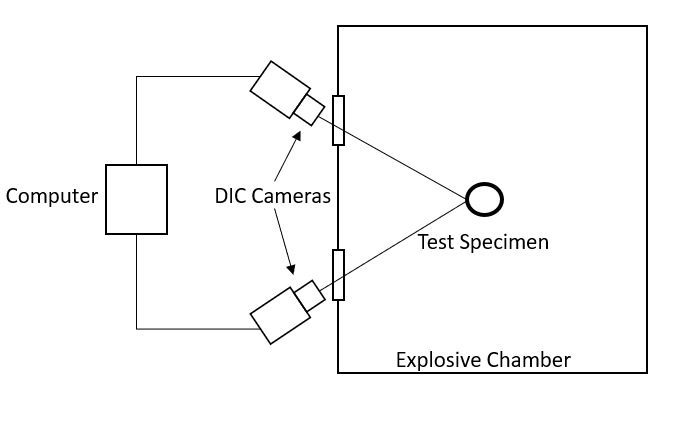
\includegraphics[width=0.7\linewidth]{Ch2/Figures/DIC_Figure.PNG}}
    \caption{Example \gls{DIC} Setup, based on illustrations from \textit{Observations in Explosive Systems with High-Speed Digital Image Correlation} \cite{DICimageObservations}}
	\label{fig:2_DIC_setup}
\end{figure}
%
%\gls{DIC} analysis begins by first calibrating the cameras to the test setup,

%DIC software overlays a colorized heat map to depict deformation at any point within the selected region of interest

%%%%%%%%%%%%%%%%%%%%%%%%%%%%%%%%%%%%
\subsection{Fragment Tracking} \label{sec:2_Fragment_tracking}
%%%%%%%%%%%%%%%%%%%%%%%%%%%%%%%%%%%%

Another useful diagnostic technique is the Matlab-based fragment tracking software developed by Daniel Guildenbecher from \gls{SNL}.


%
%-----------------------------------------------------------------------
\section{Summary} \label{sec:2_Summary}
%-----------------------------------------------------------------------
Chapter II provides a brief overview of military weaponeering limitations and how \gls{AM} presents a novel approach to custom building munitions for specific targets. It details \gls{PBF} processing and resulting material characteristics and fragmentation theories describing casing failure in explosive environments. Additionally, this chapter outlines the importance of high speed photography for investigating explosive events, and how \gls{DIC} extracts mechanical properties of test subjects. 
While experts continually look for techniques to increase weapons effectiveness while decreasing collateral damage, there is little research incorporating additively manufactured metals into explosive applications. This thesis characterizes the behavior of \gls{AM}-printed metal casings under explosive loadings, compares performance with classic fragmentation models used in weapons research, and calculates mechanical properties using visual tracking techniques.

%--------%%%%%%%------%%%%%%
%Given the previous research, I need to address...
%I will perform my research by..... (Detonating cylinders)
%I will quantify my experiments by.....

%Building on Gurney's research methodology, $L/D$ ratio was varied in the \gls{AM}-printed casings' design to induce multiple $C/M$ [data points]?? 


%Before additively manufactured metals are utilized in explosive applications, their....need to....

%This research will address by detonating.....

%DIC analysis will extract deformation and fragmentation velocities....

%This research uses fragmentation models developed by Gurney and Mott as a foundation to characterize the performance of exploding additively manufactured casings. 
